\documentclass[10pt,a4paper]{article}
\usepackage[utf8]{inputenc}
%\usepackage[french]{babel}
\usepackage[T1]{fontenc}
\usepackage{amsmath}
\usepackage{amsfonts}
\usepackage{amssymb}
\usepackage{verbatim}
\usepackage{graphicx}

\title{La télédétection et GéoBretagne : méthodes, produits et analyses}
\begin{document}

\maketitle

\begin{figure}[t!]
\centering

\includegraphics[scale=1]{img/logos.jpg}
\label{logos}
\end{figure}

\begin{abstract}
GéoBretagne a intégré des données de télédétection dans son catalogue. Dans un premier temps, 4 produits sont disponibles : 
\begin{itemize}
\item le Normalized Difference Vegetation Index (NDVI) qui est un indice de végétation mettant en valeur le dynamisme de la végétation, par sa teneur en chlorophylle et la structure du couvert végétal;
\item l'Evaporative Fraction (EF), un indice indiquant la capacité d'une surface à évaporer qu’elle soit composée de végétation, ou non. Par exemple, il représente un indicateur pour identifier des situations de stress hydrique;
\item la température moyenne sur 8 jours de jour et de nuit par temps clair;
\end{itemize}

Chacun de ces produits possède une dimension temporelle afin de suivre l'évolution de ceux-ci de manière intra et inter-annuelle. Le capteur MODIS a été choisi pour effectuer cette introduction à la télédétection.
\end{abstract}

\newpage
\tableofcontents
\newpage

\section{Introduction}

La définition officielle de la télédétection est « l’ensemble des connaissances et techniques utilisées pour déterminer des caractéristiques physiques et biologiques d’objets par des mesures effectuées à distance, sans contact matériel avec ceux-ci » (COMITAAS, 1988).\smallbreak

La notion de "sans contact matériel avec ceux-ci" correspond à l'acquisition d'informations sur la Terre à partir de satellites, avions, drones ou simplement d'un appareil photo jeté en l'air (à vos risques et périls). Pour l'étude d'autres planètes, les télescopes effectuent également de la télédétection étant donné qu'ils ne sont pas en contact avec celles-ci.\smallbreak

L'acquisition d'informations s'opère par la mesure du spectre électromagnétiques dans les domaines (figure \ref{spectreElectro}) :

\begin{itemize}
\item du visible pour l'oeil humain, comme un appareil photo
\item de l'invisible pour l'oeil humain :
\begin{itemize}
\item l'infrarouge (télécommande, capteur thermique)
\item les micro-ondes (téléphone, radar)
\end{itemize}
\end{itemize}

\begin{figure}[!h]
\centering
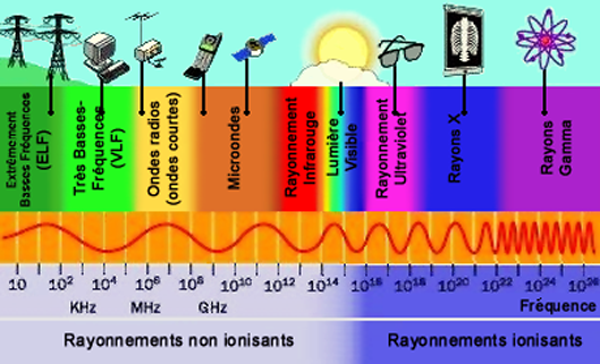
\includegraphics[scale=0.6]{img/spectre-electromagnetique.png}
\caption{Représentation du spectre électromagnétique (source : astronoo.com)}
\label{spectreElectro}
\end{figure}

Dans le cadre de cette introduction à la télédétection, les données dans les micro-ondes (radar) ne sont pas abordées.

\subsection{Capteur MODIS}

Le capteur MODIS est un spectroradiomètre imageur (un appareil photo) se trouvant sur deux satellites (Terra et Aqua) (figure \ref{modis}) mis en service par la NASA dont les données sont diffusées gratuitement.

\begin{figure}[!h]
\centering
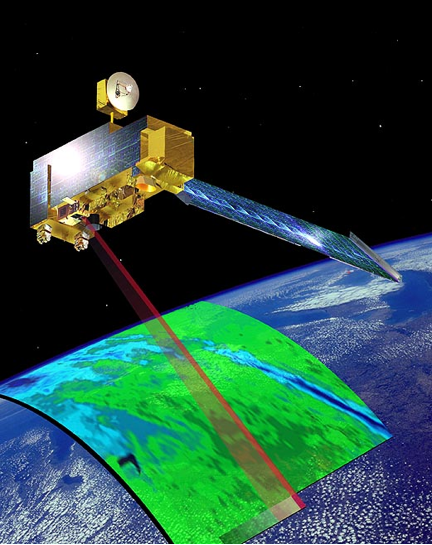
\includegraphics[scale=0.4]{img/modis.png}
\caption{Représentation du satellite Terra avec le capteur MODIS}
\label{modis}
\end{figure}

Ce capteur dispose d'une résolution spatiale allant de 250 mètres à 1 kilomètre avec une résolution temporelle journalière. Une image (tuile) de ce capteur couvre 2330 km$^2$ (figure \ref{modisGrid}).

\begin{figure}[!h]
\centering
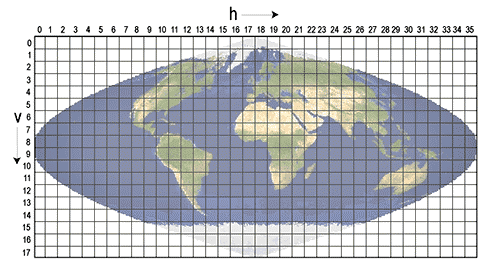
\includegraphics[scale=0.7]{img/modisGrid.png}
\caption{Grille d'acquisition des images MODIS}
\label{modisGrid}
\end{figure}

Ce capteur a été sélectionné pour plusieurs de ses caractéristiques, bien que généralement les études utilisant des images MODIS sont effectuées sur des paysages ouverts et non fragmentés en petites parcelles (Morton et al., 2006; Wardlow et al., 2006) comme la Bretagne. Celles-ci sont :
\begin{itemize}
\item des synthèses de 8 jours (valeur moyenne ou maximale, selon les produits, sur 8 jours) disponibles afin de limiter l'impact des nuages;
\item un capteur acquérant des informations dans l'infrarouge thermique (nécessaire pour calculer un indice)
\item des archives importantes permettant d'avoir des données depuis l'an 2000;
\end{itemize}

\subsection{Produits disponibles sur GéoBretagne}

Les premiers produits diffusés ont tous une dimension temporelle avec un pas de temps de 8 jours.

\subsubsection{Indice de végétation : NDVI}

Le NDVI (Rouse and Haas, 1973; Tucker, 1979) est un indice de végétation standard dans l'étude de la végétation (Gao, 1996). Cet indice se calcule avec les bandes électromagnétiques du rouge (R) et du proche infrarouge (Pir). Le résultat est normalisé entre -1 (autre que végétation tel l'eau) et 1 (végétation dynamique).\smallbreak

\begin{center}
\textrm{NDVI}=$ \frac{Pir-R}{Pir+R} $
\end{center}\smallbreak

Ces bandes sont employées d'après l’interaction des bandes du rouge et du proche infrarouge avec la végétation. L'énergie de la bande du rouge est majoritairement absorbée par la végétation (chlorophylle), au contraire du proche infrarouge qui est réfléchi principalement par l'eau contenu dans la végétation (parenchyme lacuneux). Ainsi, plus la végétation sera dynamique, plus il y aura d'absorption dans le rouge et de réflectance dans le proche infrarouge.\smallbreak

La figure \ref{signSpectr} permet de distinguer la réflectance type de la végétation (en vert), de l'eau (en bleu) et du sol (en rouge). Les bandes sont représentées par les zones grisées numérotées avec celle du rouge (3) et du proche infrarouge (4). Ainsi, le NDVI calcule la différence de réflectance entre les 2 bandes. Plus cette différence est importante (comme sur la figure \ref{signSpectr}), plus la végétation sera dynamique et le NDVI proche de 1. Concernant l'eau, sa réflectance est nulle dans le proche infrarouge, ayant pour effet d'avoir un NDVI inférieur à 0. Pour le sol, selon différents paramètres (couleur, composition, humidité, rugosité) les réflectances dans le rouge et le proche infrarouge sont équivalentes, induisant un NDVI proche de 0.\smallbreak

\begin{figure}[!h]
\centering
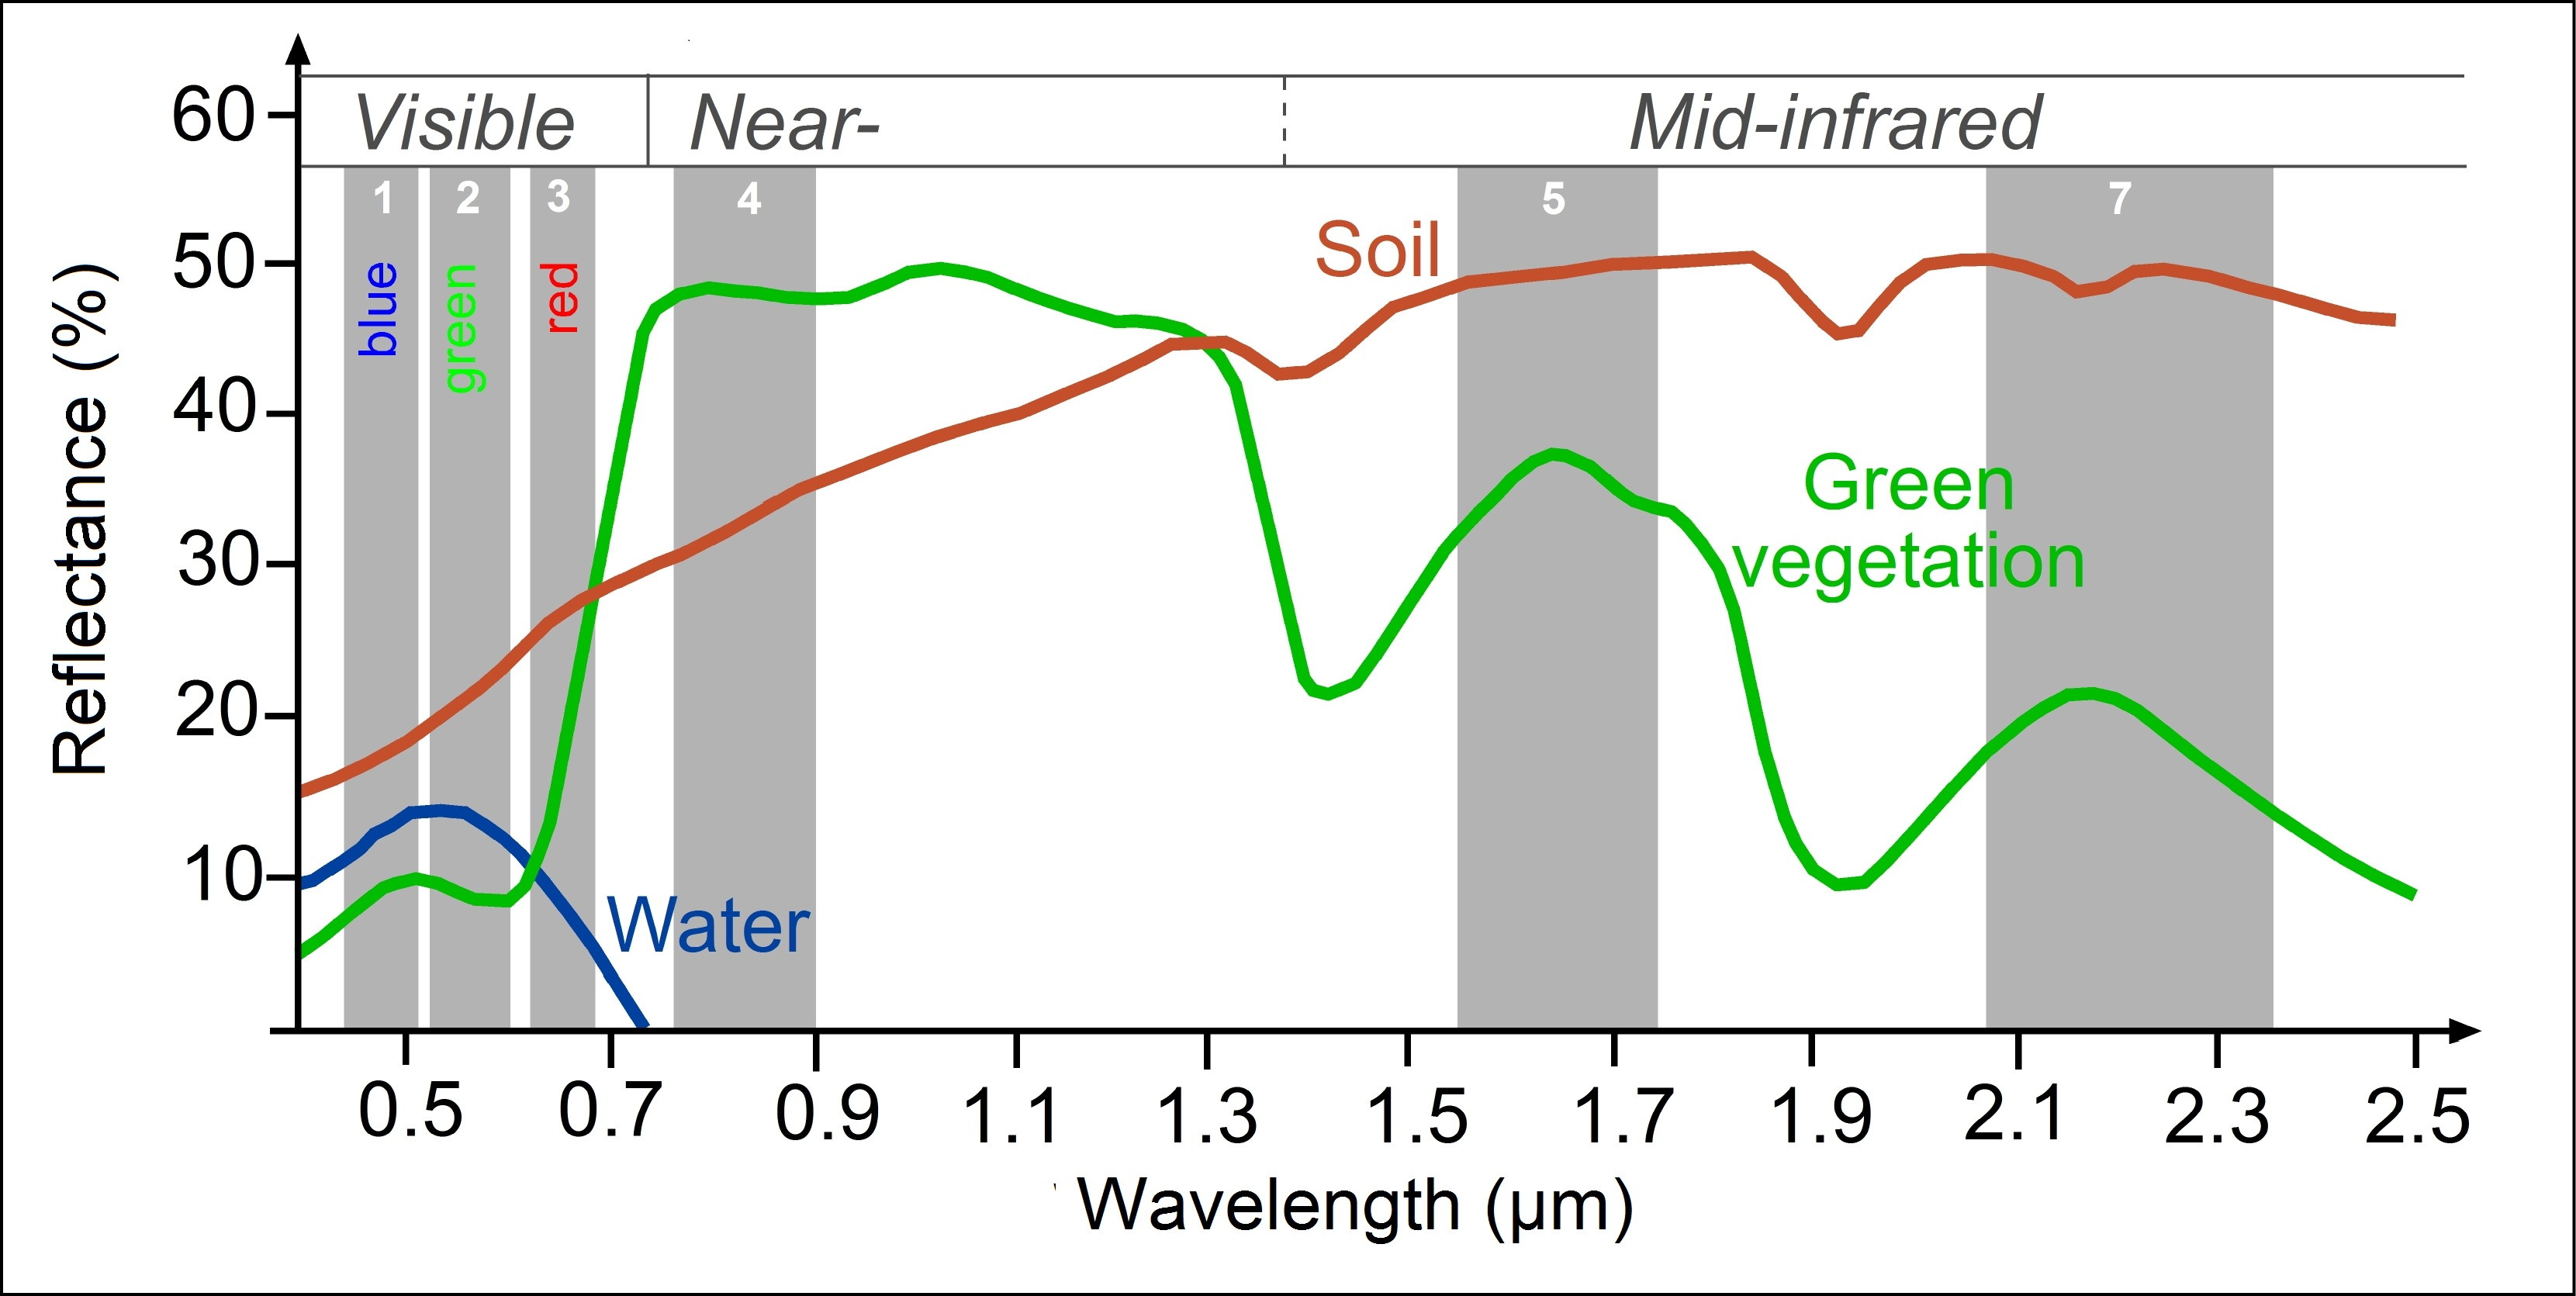
\includegraphics[scale=0.4]{img/spectral_signatures.jpg}
\caption{Signatures spectrales du sol, de l'eau et de la végétation vis à vis du spectre électromagnétique entre 350 et 2500nm. Source: SEOS Project}
\label{signSpectr}
\end{figure}

Cet indice permet par exemple d'effectuer une classification de l'occupation du sol. De part l'aspect temporel mis en avant sur GéoBretagne, cet indice permet également de suivre la phénologie de la végétation. Il est ainsi possible de déterminer l'usage des sols (Patakamuri et al., 2014).

\subsubsection{Evaporative Fraction}

L'Evaporative Fraction est un indice permettant d'estimer la capacité d'une
surface à évaporer, qu’elle soit composée de végétation ou non. Il représente ainsi un indicateur pour, par exemple, identifier des situations de stress hydrique (Bastiaanssen et al., 2003; Nutini et al., 2014). Elle est aussi une donnée servant à alimenter des modèles qui permettront l’estimation de l'évapotranspiration réelle des surfaces continentales. Cet indice se calcule avec un indice renseignant sur la couverture de la végétation (Fraction of Vegetation Cover) calculé à partir du NDVI et des mesures de températures de jour et de nuit. Les valeurs de cet indice vont de 0 (surface non évaporante) à 1.26 (surface très évaporante). Le modèle S-SEBI (Roerink et al., 2000) et le coefficient de Priestley-Taylor sont employés pour calculer EF.\smallbreak

De cette manière, il est possible de définir le stress hydrique de la végétation, particulièrement à partir d'une série temporelle (disponible sur GéoBretagne), mais aussi en combinant d'autres informations. En effet, si le sol évapore beaucoup, alors que les précipitations sont faibles, il est probable d'observer une sécheresse.

\subsubsection{Température de jour et de nuit}

Ces deux données sont téléchargeables sous la dénomination du produit MODIS MOD11A2. Ces données correspondent à la température moyenne (en kelvin) par temps clair sur 8 jours de jour et de nuit. Elles sont utilisées pour calculer EF. Ces températures sont diffusées sur GéoBretagne étant donné que plusieurs informations sont accessibles, tel les îlots de chaleur urbains avec les températures de nuit ou les milieux humides/aquatiques avec les températures de jour et de nuit étant donné leur amplitude thermique plus faible que le sol et la végétation.

\section{Méthodologie}

La chaîne de traitement développée pour générer et rendre accessible ces produits sur GéoBretagne se divise en 3 parties :

\begin{enumerate}
\item Téléchargement des images MODIS
\item Génération des produits
\item Publication des produits sur un GeoServer
\end{enumerate}

Remarque : Pour tous les produits à publier sur le Geoserver, il est impératif de respecter cette nomenclature : Nom\_YYYYMMDD.tif. Dans le cas contraire, le GeoServer (d'après un fichier de configuration) ne sera pas capable de gérer l'aspect temporel de l'image.

\subsection{Téléchargement des données MODIS}

Les produits MODIS nécessaires pour les traitements sont MOD09Q1 (bandes du rouge, du proche infrarouge et masque des nuages) à 250m de résolution spatiale et MOD11A2 (température de jour et de nuit) à 1km. La tuile à télécharger est la h17v04. Les archives pour ces produits débutent au 18 Février 2000 et une nouvelle image est ajoutée tous les 8 jours. Ces produits sont disponibles sur à cette adresse \verb!https://lpdaac.usgs.gov/data_access/data_pool.! Un compte à cette adresse \verb!https://urs.earthdata.nasa.gov/! est nécessaire pour effectuer des téléchargements. \smallbreak

Le téléchargement des images repose sur différents critères, c'est à dire le site de téléchargement, le produit, la tuile et la date dont voici le fonctionnement du script (figure \ref{orgDL}) :

\begin{figure}[!h]
\centering
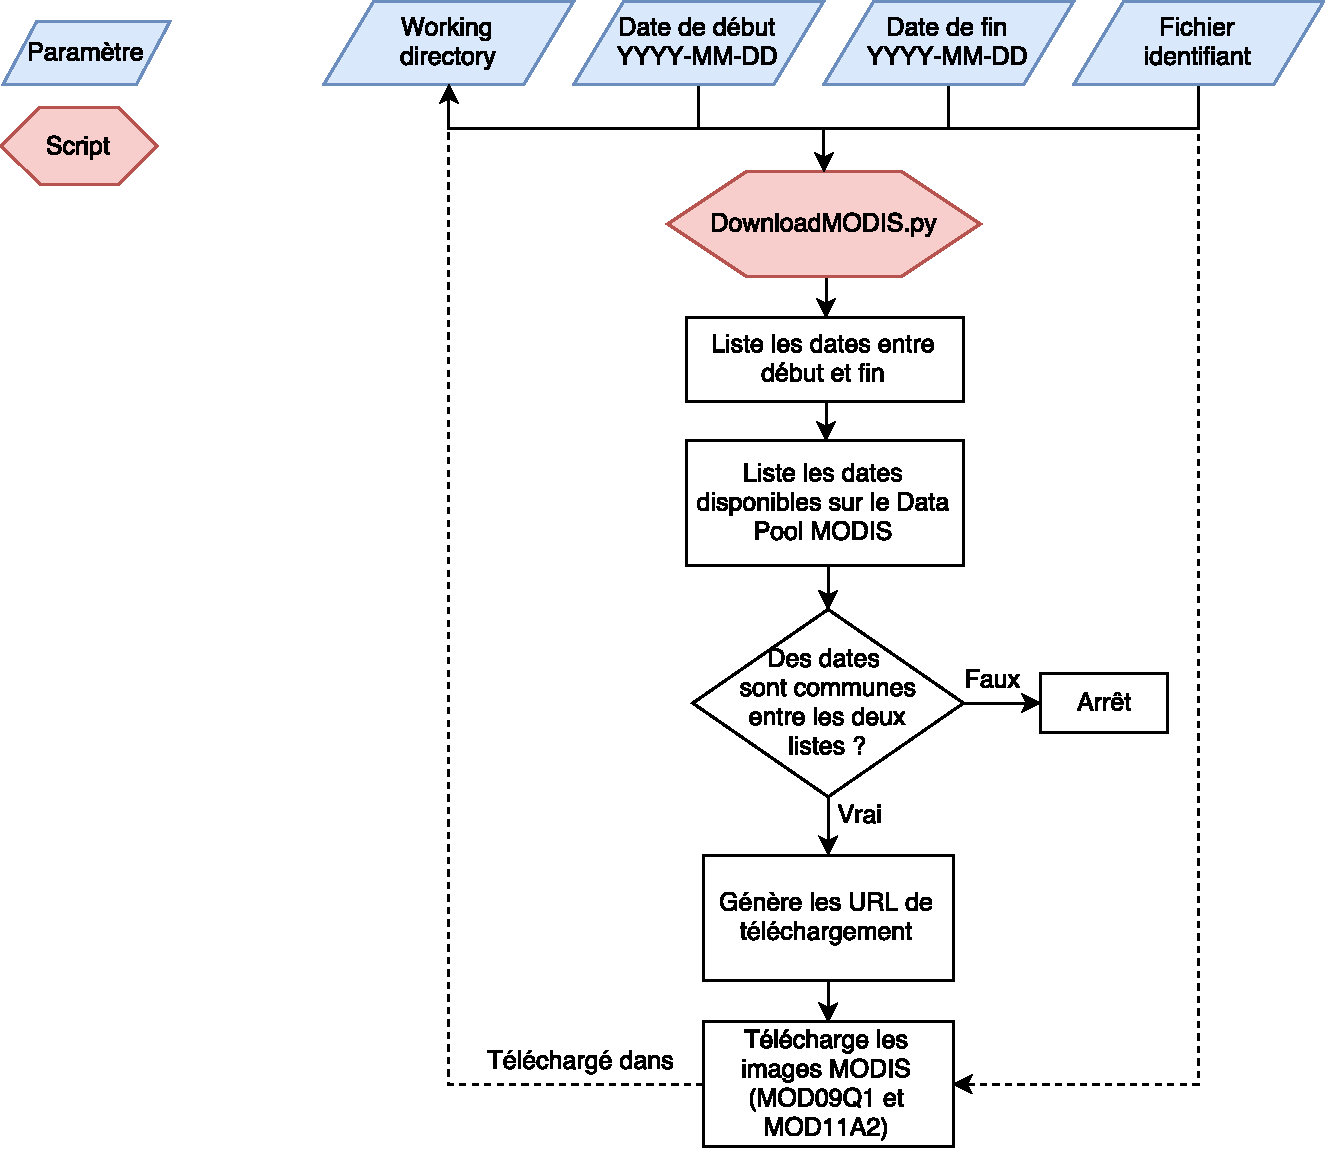
\includegraphics[scale=0.53]{img/orgDownload.pdf}
\caption{Organigramme des étapes nécessaires pour le téléchargement des produits MODIS.}
\label{orgDL}
\end{figure}

Le téléchargement s'effectue avec la requête suivante :\newline
\verb!"curl --netrc-file (1) -L -c (2).cookies -b (2).cookies (3)! \newline \verb!--output (4)"!
\begin{itemize}
\item (1) fichier contenant les identifiants pour télécharger les images
\item (2) répertoire où produire et lire un cookies concernant la session en cours (suite à une redirection)
\item (3) url du fichier à télécharger
\item (4) chemin et nom du fichier téléchargé
\end{itemize}

Les images sont téléchargées dans un répertoire nommé "usgs". Dans celui-ci se trouve les images (au format HDF) pour chacun des produits et chacune des dates, ainsi que leurs métadonnées.

\subsection{Génération des produits}

La production des produits s'opère en 4 étapes :

\begin{enumerate}
\item Prétraitement des images
\item Calcul du NDVI
\item Application de modèles
\item Calcul de l'EF
\end{enumerate}

Le fonctionnement du script pour réaliser les produits diffusés sur GéoBretagne est présenté sur la figure \ref{orgIndex}.\newpage

\begin{figure}[!h]
\centering
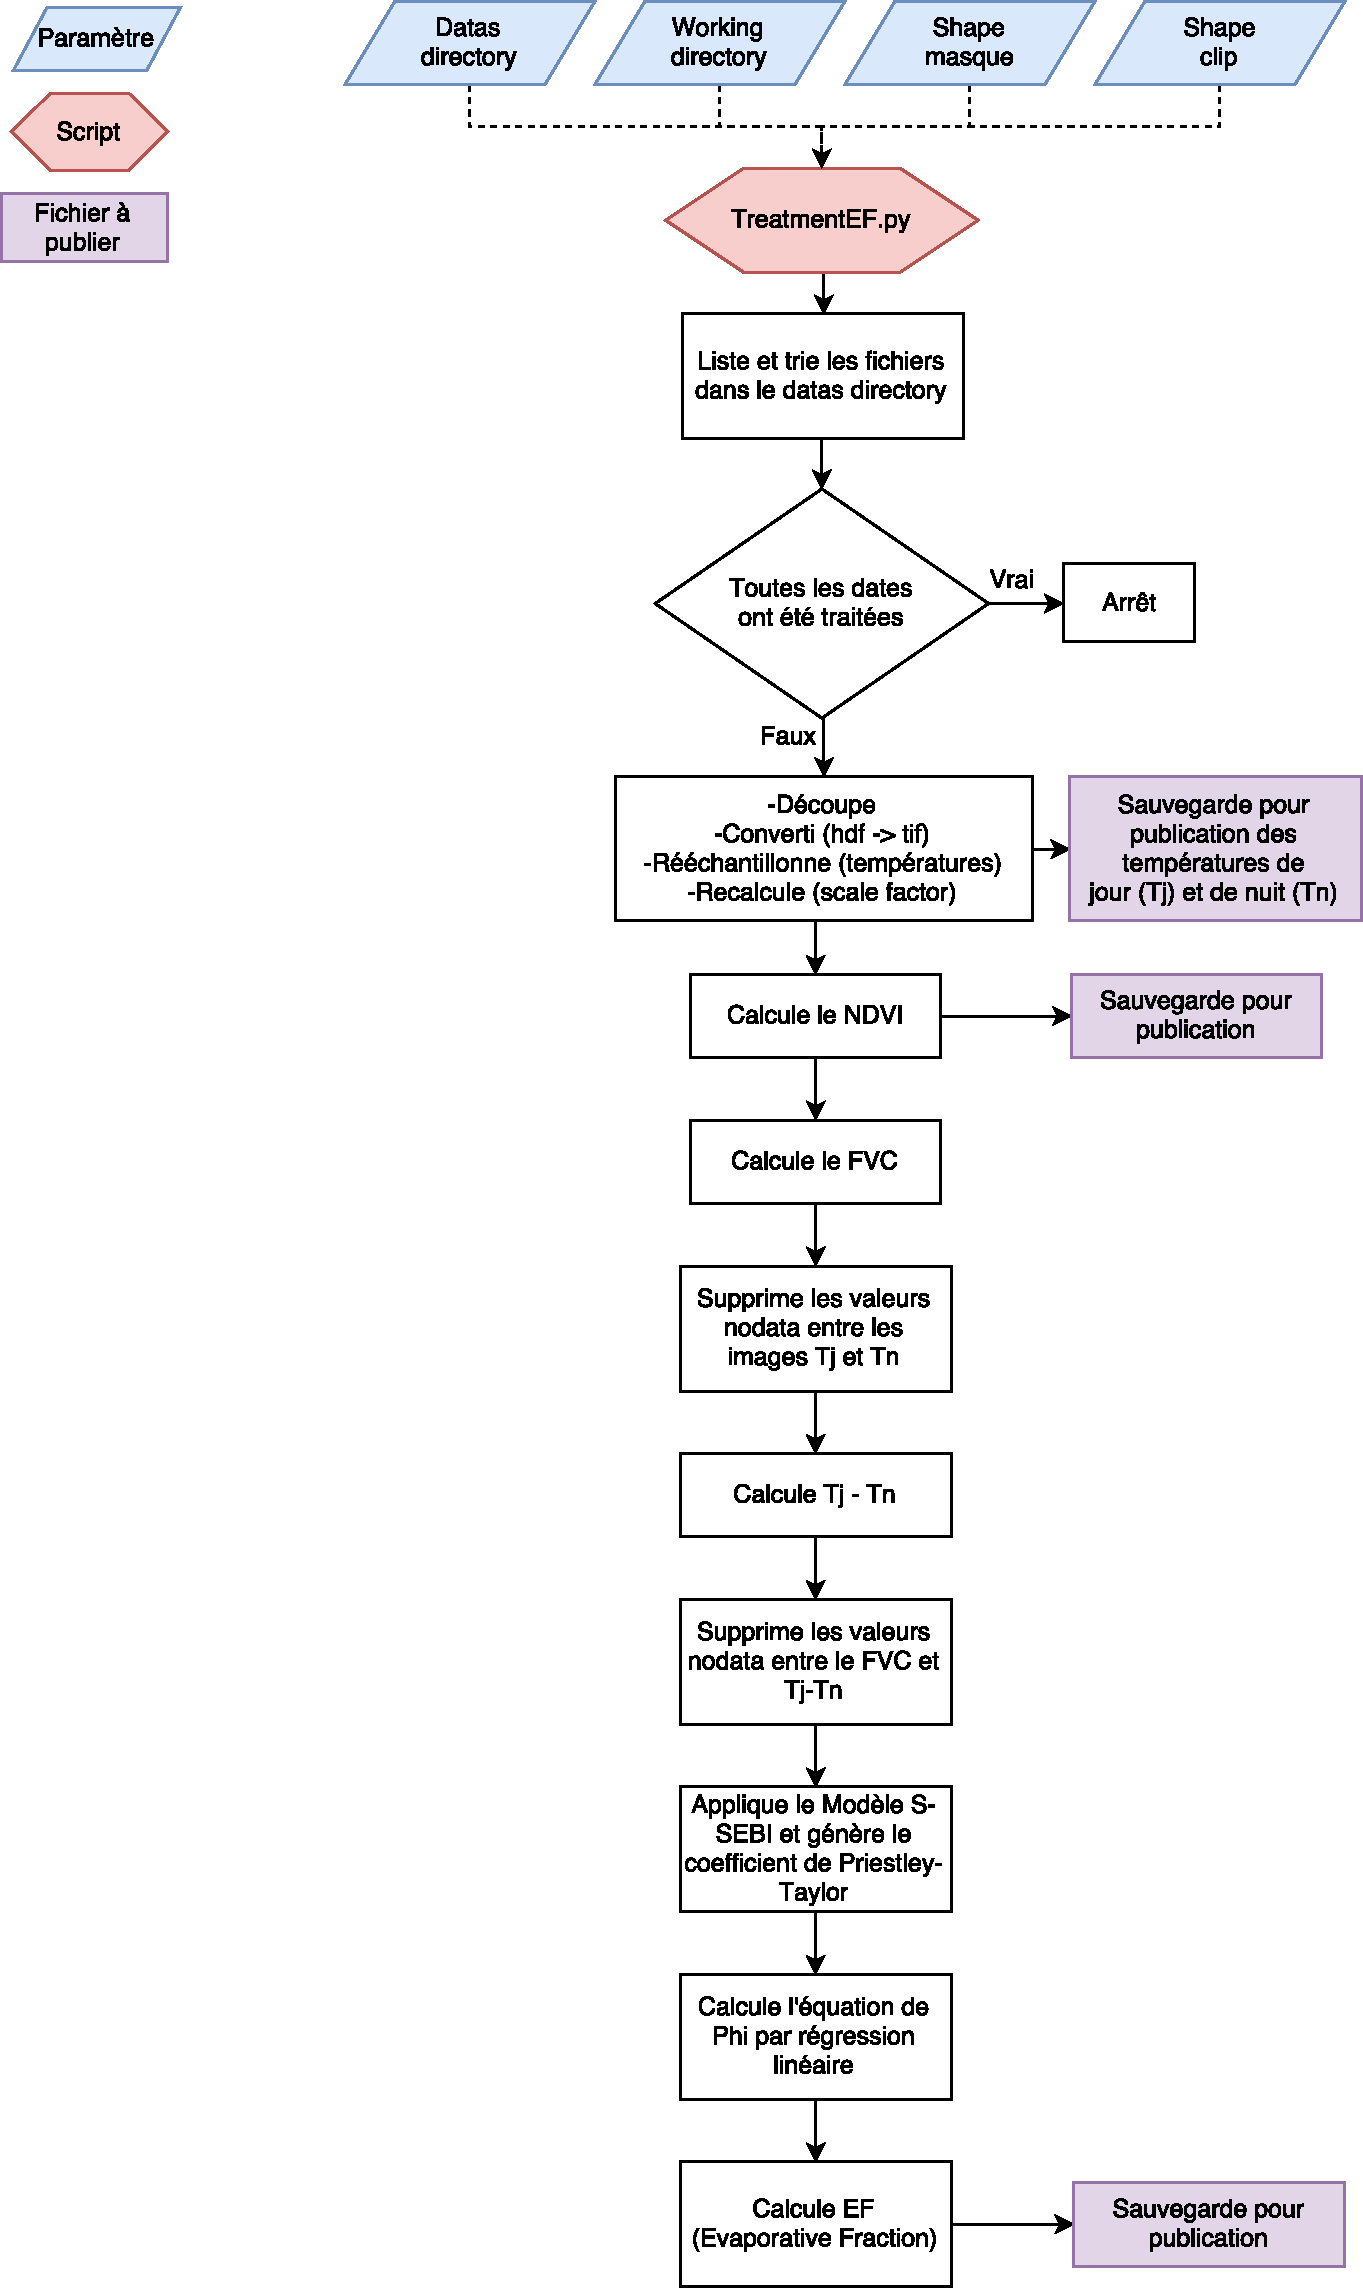
\includegraphics[scale=0.48]{img/orgIndices.pdf}
\caption{Organigramme des étapes pour la génération des indices diffusés sur GéoBretagne.}
\label{orgIndex}
\end{figure}

Tout d'abord, le script va lister tous les fichiers téléchargés. Puis, pour chaque n'ayant pas encore été traitée (test sur l'existence du fichier EF), effectue les étapes suivantes.

\subsubsection{Prétraitements}

Les images téléchargées nécessitent des prétraitements avant de générer les produits. Ils consistent à :

\begin{itemize}
\item Extraction des images : les images téléchargées sont au format HDF faisant que toutes les images d'un produit sont dans un seul fichier. Il est donc nécessaire d'extraire celles-ci. Pour cela, l'outil "\verb!gdal_translate!" est employé. 
\item Reprojection : les images sont reprojetées en Lambert 93 (epsg:2154) en respect envers la directive INSPIRE avec l'outil "\verb!gdalwarp!".
\item Découpage et masquage : les images couvrent un territoire bien plus vaste que la Bretagne et la mer ne possède pas d'informations pertinente vis à vis des indices diffusés. Il est donc nécessaire de découper les images et de supprimer les pixels de mer. Le découpage s'effectue avec un "\verb!gdalwarp! et la suppression des pixels de mer s'effectue en 3 étapes. Le première consiste à créer un raster vide de même dimension que la zone découpée, la seconde à superposer ce raster avec le fichier shape servant de masque pour faire un masque binaire avec "\verb!gdal_rasterize!". La troisième, on applique ce masque binaire pour modifier les valeurs du fichier .TIF.
\item Rééchantillonnage : les deux produits téléchargés ont une résolution spatiale différente, il n'est donc pas possible de les superposer. Un rééchantillonnage est donc nécessaire. Les températures avec 1km de résolution sont donc rééchantillonnées à 250m.
\item Recalcul des valeurs : pour une raison de stockage, les images téléchargées ont des valeurs entières. Un facteur d’échelle à appliquer à tous les produis est accessible sur le site de la LP DAAC pour obtenir les réflectances.
\item Suppression des nuages : malgré le fait que ce sont des synthèses de 8 jours qui sont utilisées pour générer les produits diffusés sur GéoBretagne, des nuages peuvent subsister. Dans un soucis de compréhension simplifié, il a été décidé qu'il était préférable de diffuser des zones sans données. Ainsi, d'après l'image qualité disponible dans le produit MOD09Q1, toutes les valeurs en dessous de 220 sont conservées.
\end{itemize}

\subsubsection{NDVI}

L'étape suivante consiste à calculer le NDVI. Pour calculer EF, les valeurs inférieures à 0 et supérieures à 1 (quelques pixels de mer non masqués ayant des valeurs aberrantes) sont supprimés. Ce changement de valeurs n'est pas répercuté sur le produit NDVI diffusé sur GéoBretagne.

\subsubsection{Modèle S-SEBI et coefficient Priestley-Taylor}

Pour pouvoir appliquer le modèle S-SEBI et générer le coefficient de Priestley-Taylor, il est nécessaire de calculer le Fractional Vegetation Cover (FVC) et calculer la température de surface (figure \ref{graphFVCTemp}).

\begin{figure}[!h]
\centering
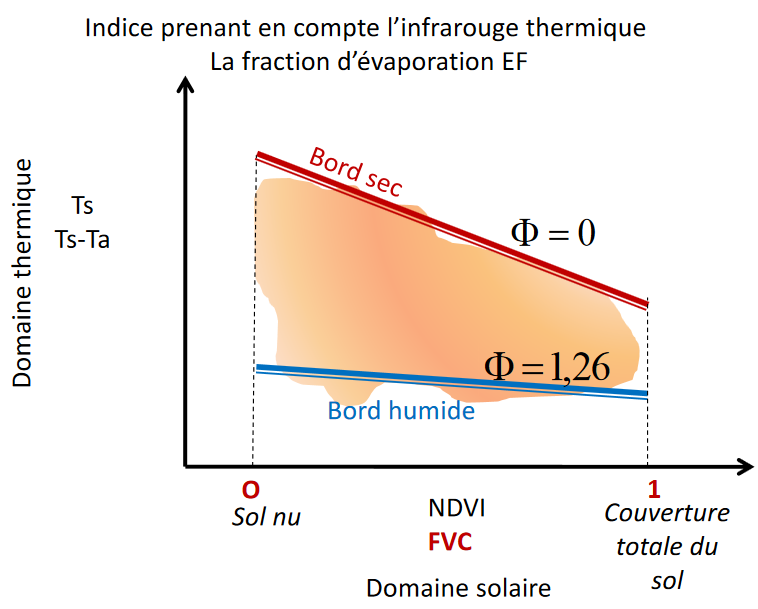
\includegraphics[scale=0.35]{img/graph_fvc_temp.png}
\caption{Graphique représentant le modèle S-SEBI pour générer le coefficient de Priestley-Taylor afin de calculer l'Evaporative Fraction.}
\label{graphFVCTemp}
\end{figure}

\begin{enumerate}
\item[(a)]FVC \medbreak
Cet indice représente la couverture de la végétation sur le sol. Plus l'indice est proche de 1, plus le sol est recouvert par la végétation et inversement. Il se calcule de la manière suivante :
\begin{center}
\textrm{FVC}=$ (\frac{NDVI-minNDVI}{maxNDVI-minNDVI})^2 $
\end{center}\smallbreak

\item[(b)]Température Tj - Tn \medbreak
Pour calculer cette valeur, il est d'abord nécessaire de reporter les pixels sans données d'une image sur l'autre. Si cette étape n'est pas effectuée, des températures aberrantes vont être générées suite à la soustraction. Ces pixels sans données seront également à supprimer sur le FVC avant d'opérer le traitement suivant.
\end{enumerate}

Avec le FVC et l'image Tj - Tn, nous pouvons produire le nuage de point des valeurs (figure \ref{graphFVCTemp}) et récupérer uniquement les points composant les bords sec et humides pour calculer le coefficient de Priestley-Taylor. Ce coefficient ainsi que l'équation de droite associé sont obtenus après une double interpolation pour ces deux bords suivis d'une régression linaire entre eux (figure \ref{graphPriestley}).

\begin{figure}[!h]
\centering
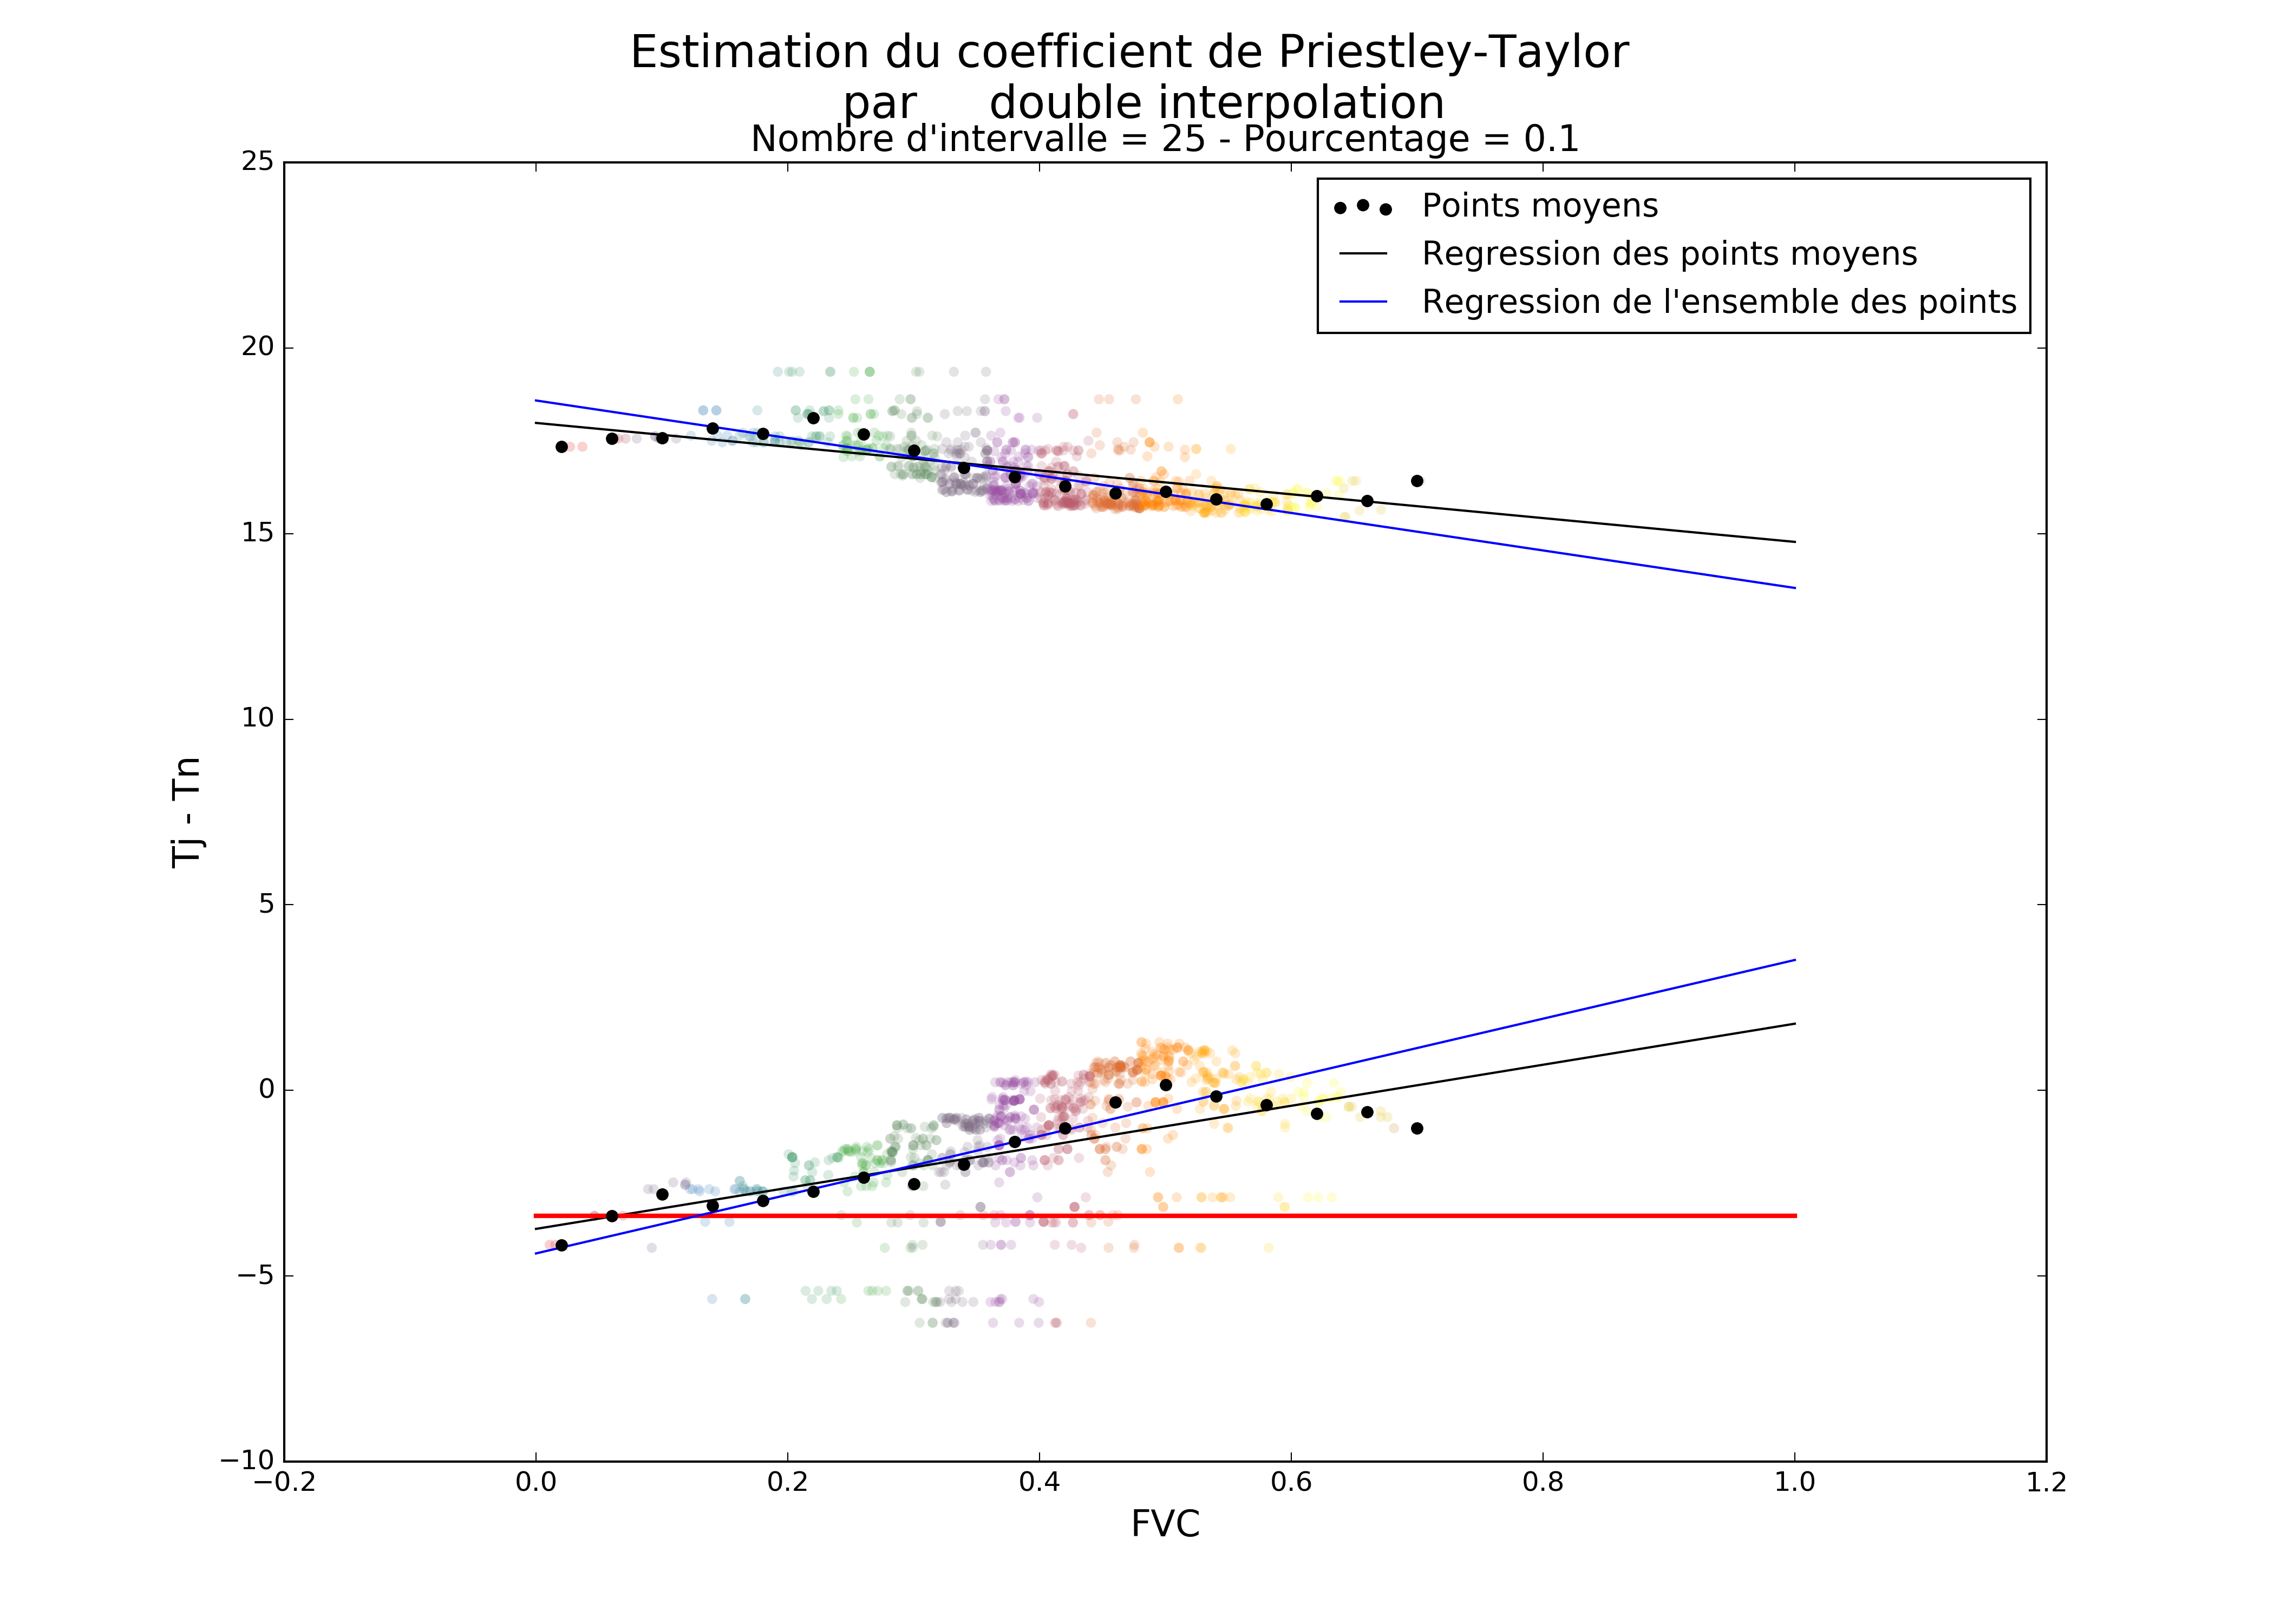
\includegraphics[scale=0.35]{img/graph_priestley.png}
\caption{Estimation du coefficient de Priestley-Taylor par double interpolation afin de calculer l'Evaporative Fraction.}
\label{graphPriestley}
\end{figure}

\subsubsection{Evaporative Fraction}

Le calcul de cet indice se déroule en plusieurs étapes :
\begin{enumerate}
\item Calcul de la température maximale d'après l'équation de droite obtenue précédemment
\item Avec cette température, calcul du coefficient de Priestley-Taylor :
\begin{center}
\textrm{Phi}=$ (\frac{Tmax-TjTn}{Tmax-Tmin})*1.26 $
\end{center}\smallbreak
\item Calcul de la température moyenne :
\begin{center}
\textrm{Tmoy}=$ ({Tj+Tn})/2 $
\end{center}\smallbreak
\item Calcul de ESatTa :
\begin{center}
\textrm{ESatTa}=$ (1000*exp(52.57633-(\frac{6790.4985}{Tmoy})-5.02808*log(Tmoy))) $
\end{center}\smallbreak
\item Calcul de delta :
\begin{center}
\textrm{delta}=$ (\frac{ESatTa}{Tmoy}) * ((\frac{6790.4985}{Tmoy})-5.02808) $
\end{center}\smallbreak
\item Calcul de EF :
\begin{center}
\textrm{EF}=$ (\frac{delta}{(delta+66)})*Phi $
\end{center}\smallbreak
\end{enumerate}

Nous obtenons une image renseignant sur la capacité d'un sol à évaporer. L'étape suivante consiste à publier ces données sur un GeoServer.

\subsection{Publication des produits sur un GeoServer}

\subsubsection{Initialisation du workspace, du store et du répertoire de données pour des données temporelles}

Ci-dessous la démarche à adopter pour générer un store temporel avec des données formalisés pour celui-ci.

\begin{enumerate}
\item Création du workspace en nommant celui-ci.
\item Copier les images sur le GeoServer si elles n'ont pas été produites sur celui-ci. De plus, ajouter dans ce dossier deux fichiers de configurations pour exploiter la dimension temporelle des images :
\begin{itemize}
\item indexer.properties avec :
\begin{itemize}
\item TimeAttribute=time (nom de l'attribut temporel)
\item ElevationAttribute=elevation (dans le cas d'une dimension altitudinale)
\item \verb!Schema=*the_geom:Polygon,location:String,!\newline \verb!time:java.util.Date,elevation:Integer!
\item PropertyCollectors=TimestampFileNameExtractorSPI \newline [timeregex](time)
\end{itemize}
\item timeregex.properties avec :
\begin{itemize}
\item regex=[0-9]{8} (pour indiquer que la date est au format YYYYMMDD)
\end{itemize}
\end{itemize}
\item Création du store avec l'extension ImageMosaic et en indiquant le répertoire contenant les images et les deux fichiers de configuration.
\item Création du layer en renseignant :
\begin{itemize}
\item onglet Data : dans la cellule sorting "time D" pour trier les dates (time correspondant au nom de l'attribut indiqué dans indexer.properties) par ordre décroissant (D)
\item onglet Dimensions : activer le time et choisir une présentation "List"
\end{itemize}
\item Le store temporel est configuré, la mise à jour passera par un script.
\end{enumerate}

Ces étapes sont à effectuer manuellement.

\subsubsection{Mise à jour d'un store temporel existant}

Un script effectue cette étape et possède 5 paramètres en entrée :

\begin{itemize}
\item l'url du Geoserver
\item le workspace du produit
\item le store du produit
\item un fichier d'identifiant pour le GeoServer
\item le répertoire sur le serveur contenant le produit à publier
\end{itemize}

Ce script publie un seul produit à la fois, il est donc à exécuter autant de fois que nécessaire.\newpage

\begin{figure}[!h]
\centering
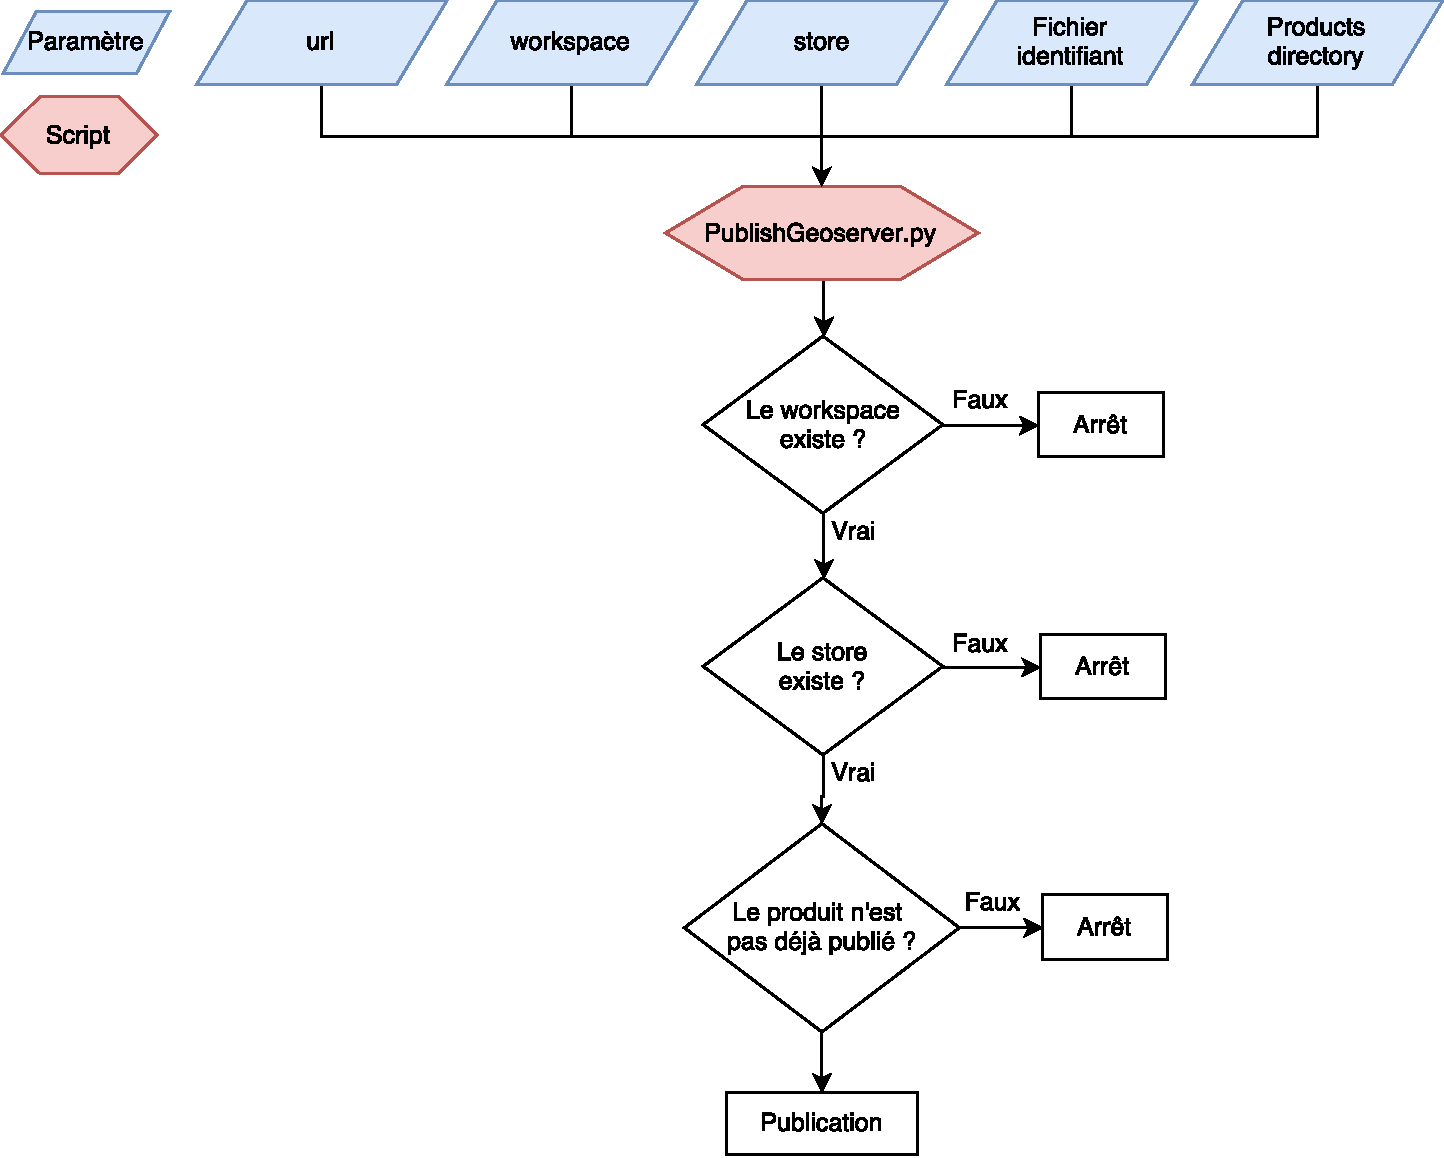
\includegraphics[scale=0.5]{img/orgPublication.pdf}
\caption{Organigramme des étapes pour la publication des indices sur un GeoServer.}
\label{orgPublication}
\end{figure}

Ainsi, la publication passe par plusieurs test afin de contrôler si le workspace, le store et la couche existent déjà (figure \ref{orgPublication}). Dans les deux premiers test, il n'est pas possible de publier la couche en leur absence et le troisième test évite de publier plusieurs fois la même image.\smallbreak
Si les tests sont réussis, alors cette commande est exécutée pour publier l'image :\newline 
\verb!"curl -v -u login:password -XPOST -H 'Content-type: text/plain'!\newline \verb!-d 'file://data/XX_YYYYMMDD.tif' 'http://geoserver/rest!\newline \verb!/workspaces/workspace/coveragestores/store/external.imagemosaic'"!

\section{Exemples d'interprétation des produits}

Ce chapitre a pour objectif de présenter l'interprétation de chacun des produits diffusés.

\subsection{Interprétation du NDVI}

Le NDVI est un indice de végétation permettant de déterminer l'occupation du sol. D'après le fonctionnement de cet indice (1.2.1), il est possible de distinguer sur la figure \ref{NDVI1} les espaces forestiers avec un NDVI élevé, la ville de Rennes avec un NDVI nul et l'embouchure de la Loire avec des valeurs négatives.

\begin{figure}[!h]
\centering
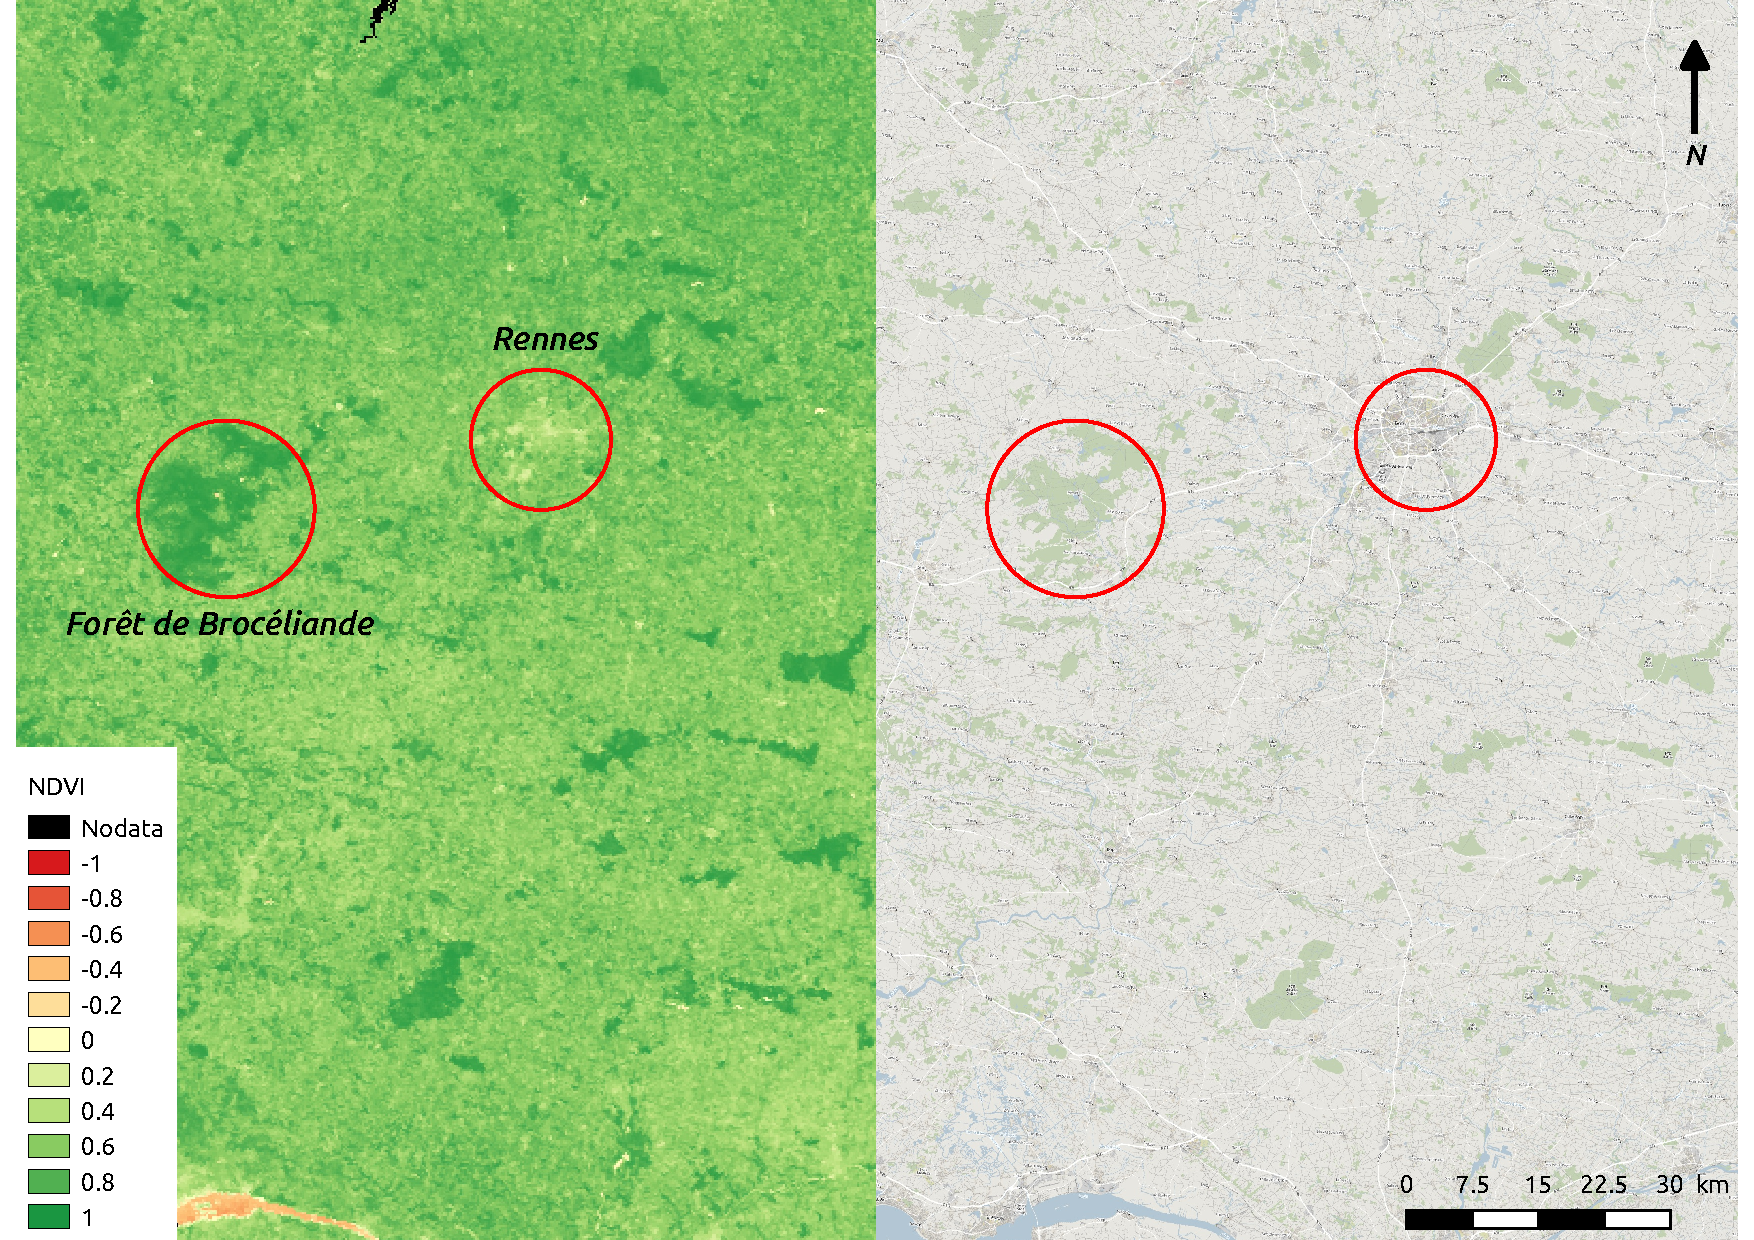
\includegraphics[scale=0.33]{img/NDVI_interpretation1.pdf}
\caption{NDVI au 18 Juin 2017 (à gauche) permettant de distinguer les espaces forestiers, la ville de Rennes et l'embouchure de la Loire.}
\label{NDVI1}
\end{figure}

\subsection{Interprétation de l'évolution temporelle du NDVI}

L'intérêt d'une série temporelle est de pouvoir suivre l'évolution d'un phénomène. Dans le cadre de cet exemple, nous allons observer l'évolution du NDVI sur le marais du Parc Naturel Régional de Brière. Avant tout, à cause des nuages, certaines dates ne disposent pas d'informations sur le PNR. Ce manque de données s'identifie par des ruptures dans la courbe de la figure \ref{TS_NDVI}.\smallbreak
Cette courbe présente globalement une forme sinusoïdale correspondant aux saisons de végétations (croissance, stagnation, diminution). Ces différentes étapes peuvent être décalée dans le temps selon les objets observés. Par exemple, une culture de blé aura une phase de croissance à partir de novembre-décembre (tallage) au contraire d'une prairie où la croissance s'effectuera à partir de mars.\smallbreak
La série temporelle accessible sur GéoBretagne présente l'avantage de couvrir différents aléas comme la canicule de 2003. Pour cet exemple, 2 années ont été sélectionnées avant et après celui-ci (figure \ref{TS_NDVI}).\smallbreak
Sur le marais du PNR de Brière, cet aléa ne se distingue pas vis à vis des autres années, probablement pour deux raisons :
\begin{itemize}
\item le marais, ayant une réserve en eau importante, a su conserver un niveau correct durant la canicule induisant aucun impact sur la végétation
\item l'arrêt du traitement chimique visant à éliminer la Jussie, en plus de la canicule, a considérablement accéléré le développement de la Jussie (Leplat M., 2005), raison pour laquelle nous n'observons aucune diminution du NDVI
\end{itemize}
Cependant, d'autres éléments peuvent expliquer l'absence de l'impact de la canicule, par exemple, la définition même de la canicule. En France, une canicule à Brest se situe à 28 degrés, alors qu'une canicule à Toulouse se situe à 36 degrés.\smallbreak
Dans tous les cas, pour effectuer un suivi temporelle sur des objets, il est important de prendre en compte l'occupation et l'usage des sols qui en est fait chaque année. Par exemple, dans le cas de parcelles agricoles, il est primordial de prendre en compte la rotation des cultures pour effectuer une analyse pertinente.

\begin{figure}[!h]
\centering
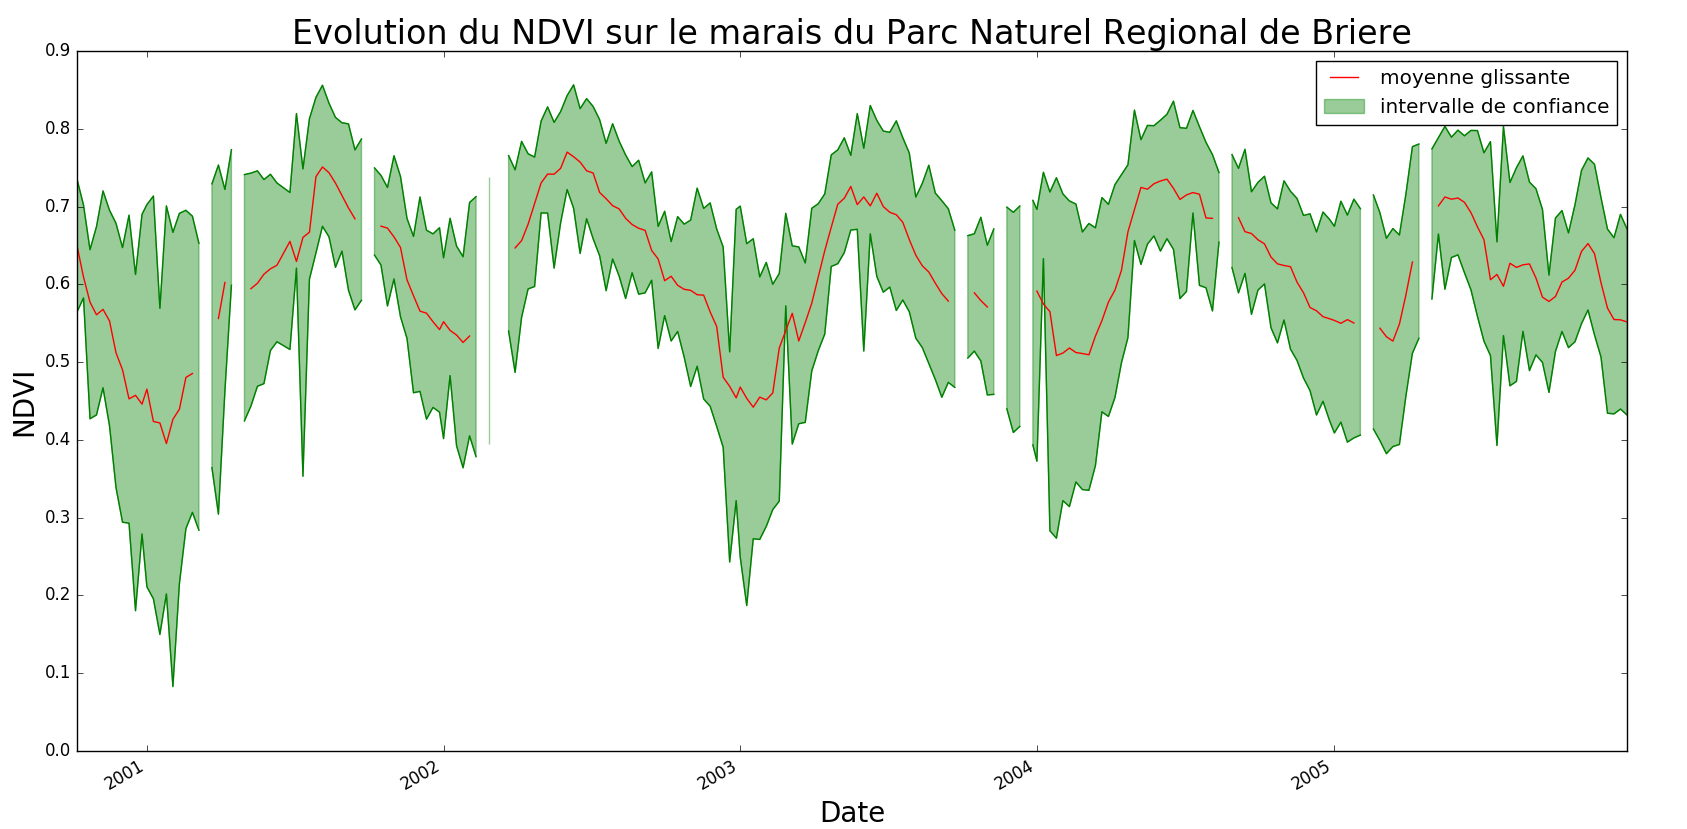
\includegraphics[scale=0.29]{img/NDVI_Briere.png}
\caption{Représentation de l'évolution du NDVI entre 2000 et 2017 sur le Parc Naturel Régional de Brière.}
\label{TS_NDVI}
\end{figure}

\subsection{Interprétation de l'Evaporative Fraction}

EF est un indice renseignant sur la capacité d'une
surface à évaporer, qu’elle soit composée de végétation ou non. D'après la figure \ref{EF1}, la moitié sud de l'image évapore peu, sauf quelques endroits correspondants aux espaces forestiers et au Parc Naturel Régional (PNR) de Brière. Ainsi, ne pas observer cette différence d'évaporation signifierai un stress hydrique important mettant en péril ces espaces.

\begin{figure}[!h]
\centering
\includegraphics[scale=0.33]{img/EF_interpretation1.pdf}
\caption{Evaporative Fraction au 18 Juin 2017 (à gauche) permettant de distinguer les espaces forestiers et le PNR de Brière et d'estimer le stress hydrique.}
\label{EF1}
\end{figure}

\newpage 

\subsection{Interprétation des températures de jour}

La température de jour correspond à la température moyenne sur 8 jours par temps clair. Cette mesure, en kelvin, est un produit diffusés par l'USGS sous le terme MOD11A2. Cette donnée est nécessaire pour calculer EF. Compte-tenu des éléments discernables (zones humides, forêts, zones urbaines) à partir de cette température (figure \ref{TJ1}), il a été décidé de mettre à disposition cette information. \smallbreak

\begin{figure}[!h]
\centering
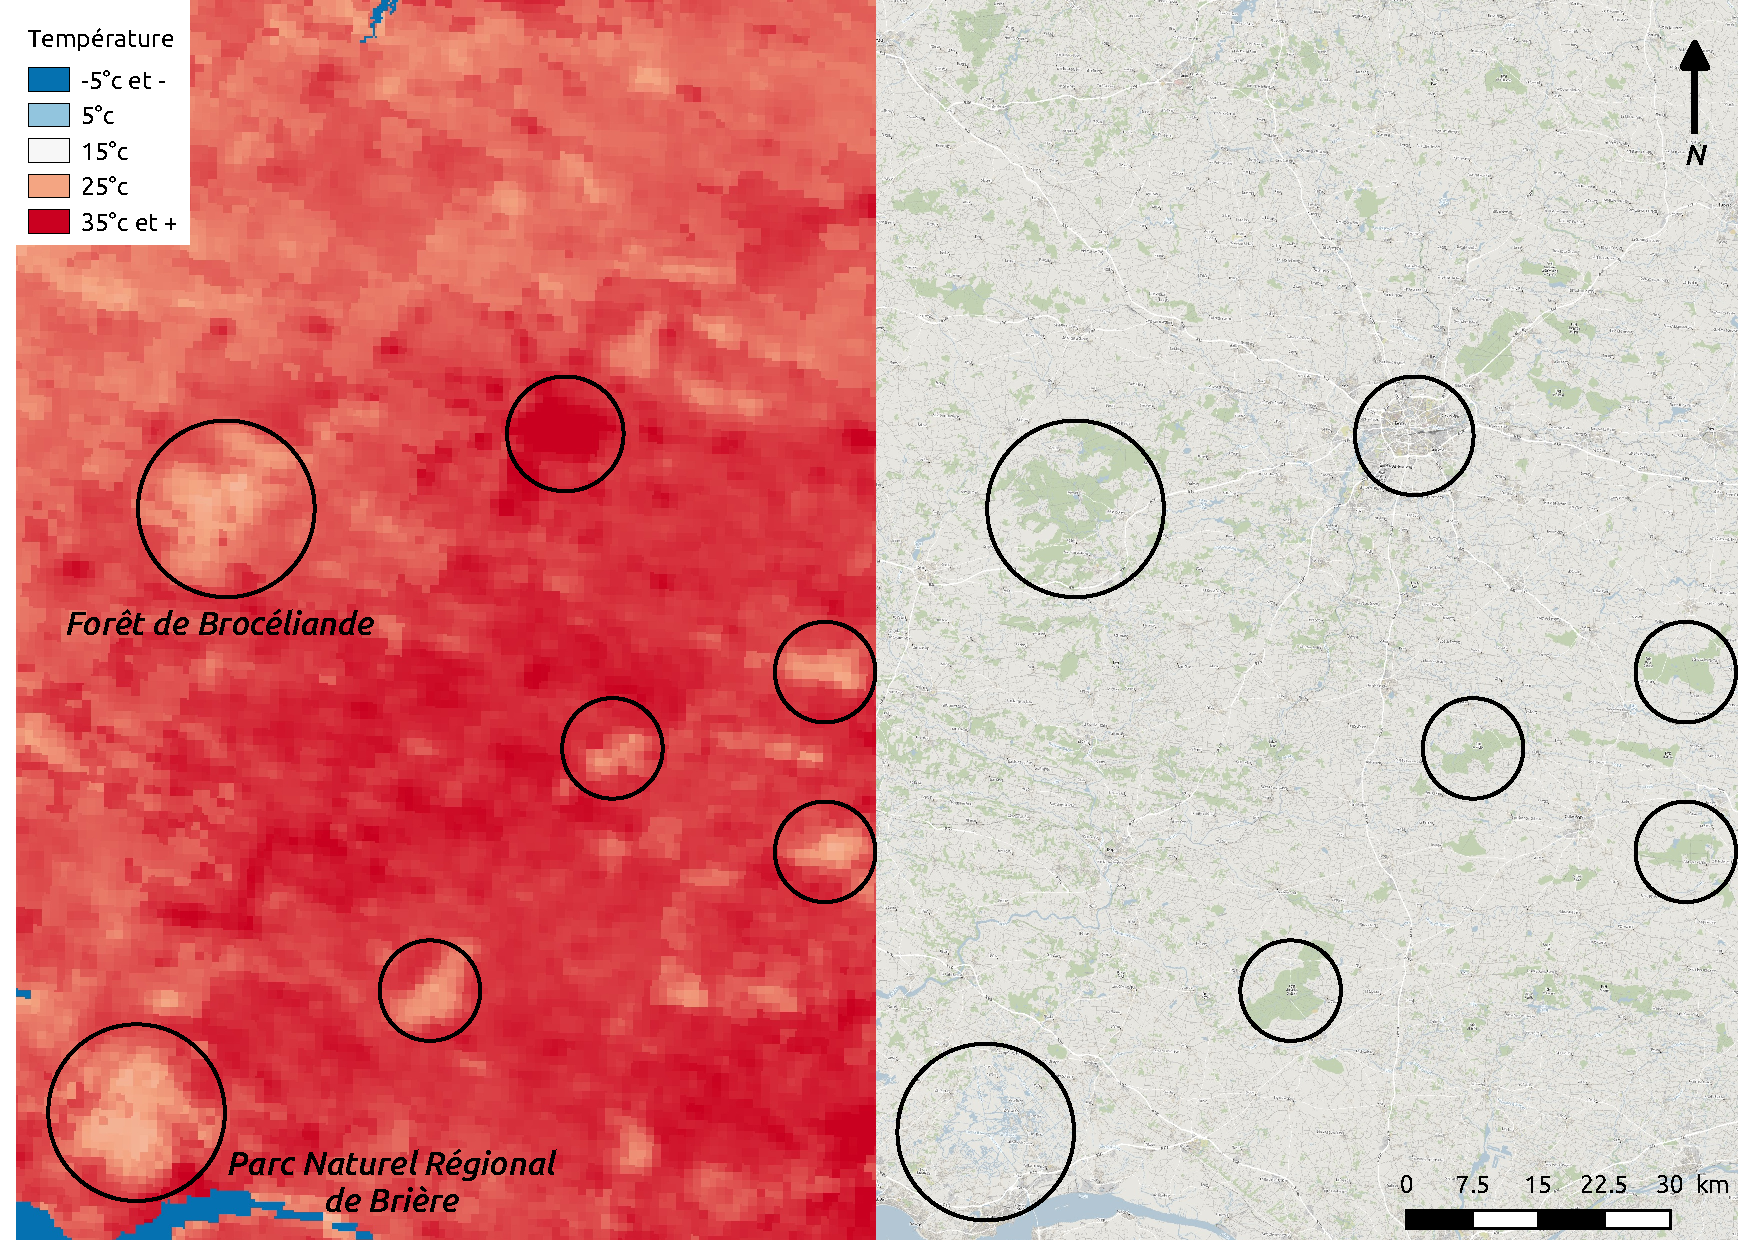
\includegraphics[scale=0.33]{img/TJ_interpretation1.pdf}
\caption{Température de jour au 18 Juin 2017 (à gauche) permettant de distinguer les espaces forestiers, le PNR de Brière et Rennes.}
\label{TJ1}
\end{figure}

\subsection{Interprétation des températures de nuit}

La température de nuit correspond à la température moyenne sur 8 jours par temps clair. Cette mesure, en kelvin, est un produit diffusés par l'USGS sous le terme MOD11A2. Cette donnée est nécessaire pour calculer EF, et compte-tenu des éléments discernables (principalement les îlots de chaleur urbains tel que Rennes) à partir de cette température (figure \ref{TN1}), il a été décidé de mettre à disposition cette information. \smallbreak 

\begin{figure}[!h]
\centering
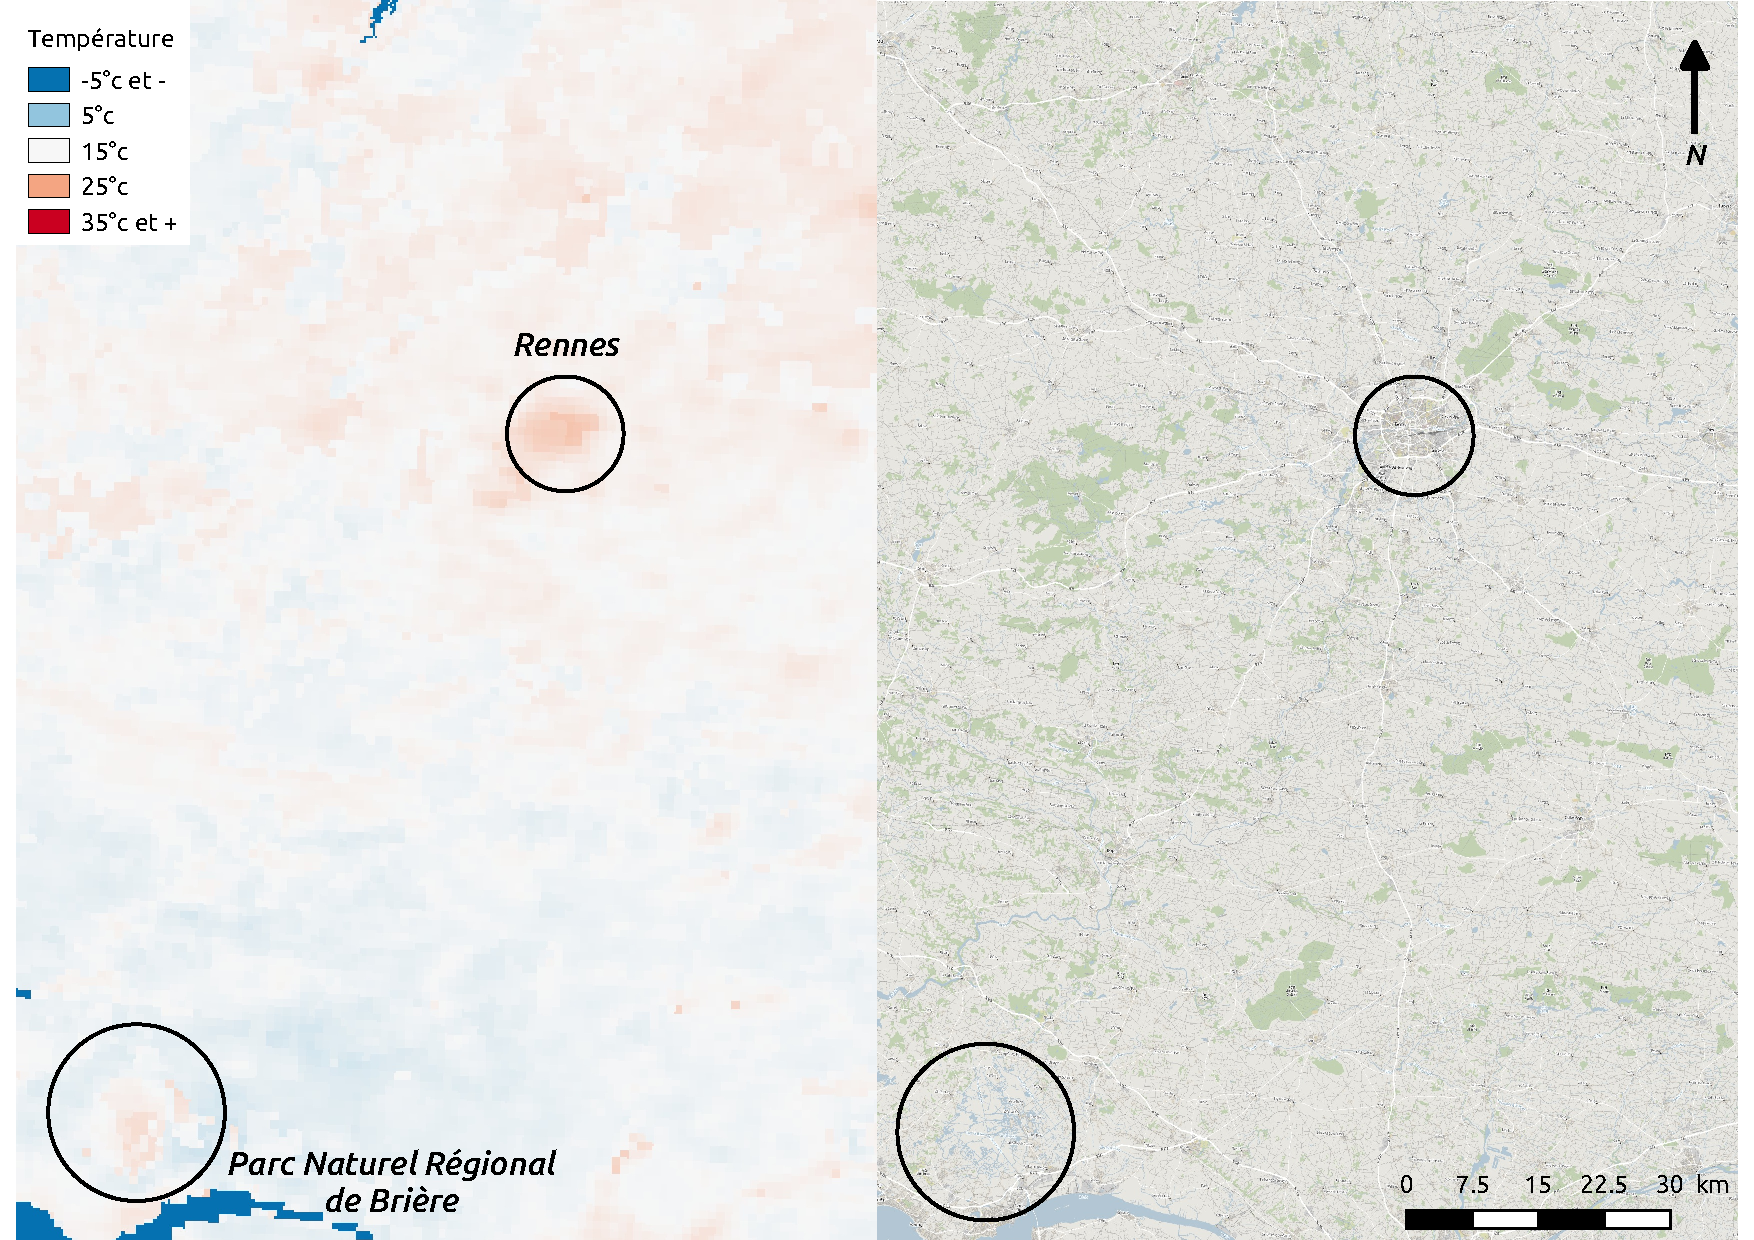
\includegraphics[scale=0.33]{img/TN_interpretation1.pdf}
\caption{Température de nuit au 18 Juin 2017 (à gauche) permettant de distinguer la ville de Rennes (îlot de chaleur urbain) et le PNR de Brière.}
\label{TN1}
\end{figure}

\section{Conclusion}

La télédétection est un outil permettant d'acquérir des informations invisibles à l’œil nu sans avoir besoin d'aller sur le terrain pour les acquérir. Elle permet également d'optimiser ces enquêtes nécessitant du personnel et coûteuses en temps. Il est donc possible d'effectuer un suivi sur un paysage ou tout autre éléments composant la biosphère à moindre coût. En effet, certains phénomènes ne peuvent être décrit et compris sans cette dimension (déforestation, urbanisation, érosion).\smallbreak
GéoBretagne souhaite donc rendre accessible nombre de ces informations pour permettre d'optimiser les études effectués en Bretagne en fournissant des produits permettant de répondre aux problématiques actuelles et futures du territoire.\smallbreak

\section{Perspectives}

Les produits diffusés actuellement sur GéoBretagne possèdent plusieurs limites :
\begin{itemize}
\item la résolution spatiale de MODIS n'est pas adaptée au paysage Breton particulièrement fragmenté. Il n'est donc pas possible d'observer les bosquets, petites parcelles et les haies, entre autres. Il est donc envisagé d'utiliser le capteur Landsat (résolution spatiale de 30 mètres et une bande dans l'infrarouge thermique (critère obligatoire)).
\end{itemize}

\section{Bibliographie}

\begin{itemize}
\item Bastiaanssen W.G.M., Ali, S. (2003). "A new crop yield forecasting model based on satellite measurements applied across the Indus Basin, Pakistan". Agric. Ecosyst. Environ. 94, pp.321–340.
\item Gao B.-C. (1996). "NDWI : A  Normalized  Difference  Water  Index  for  remote  sensing  of vegetation liquid water from space", Proceeding of SPIE.Vol.58, no.3, pp.257-266.
\item Leplat Mélody.(2005). "Les proliférations de Jussies sous l'angle économique". Mémoire. Université de Bretagne occidentale - Agrocampus Rennes
\item Morton, D. C., DeFries, R. S., Shimabukuro, Y. E., Anderson, L. O., Arai, E., del Bon Espirito-Santo, F.,  Freitas,  R.  et  Morisette,  J.,  (2006). "Cropland expansion changes deforestation dynamics in the southern Brazilian Amazon", Proceedings of the National Academy of Sciences, 103(39):14637. 
\item Nutini F., Boschetti M., Candiani G., Bocchi S., Brivio P.A., (2014). "Evaporative Fraction as an indicator of moisture condition and water stress status in semi-arid rangeland ecosystems". Remote sens., 6, pp.6300-6323.
\item Patakamuri S.K., Agrawal S., Krishnaveni M. (2014). "Time-series analysis of MODIS NDVI data along with ancillary data for land use/land cover mapping of Uttarakhand". The International Archives of the Photogrammetry, Remote Sensing and Spatial Information Sciences. XL-8, ISPRS Technical Commission VIII Symposium, pp.1491–1500
\item Roerink G., Su Z., Menenti M. (2000). "S-SEBI: A simple remote sensing algorithm to estimate the surface energy balance". Phys. Chem. Earth Part B 25, pp.147–157.
\item Rouse and Haas, (1973). "Monitoring vegetation systems in the great plain with ERTS", Third ERTS Symposium, Washington DC: NASA, no.1, pp.309-317.
\item Tucker, (1979). "Red and photographic infrared linear combinations for monitoring vegetation", Remote Sensing of the Environment, no.8, pp.127–150. 
\item Wardlow, B.D., Kastens, J.H. et Egbert, S.L. (2006). "Using USDA crop progress data for the evaluation of greenup onset date calculated from MODIS 250meter data", Photogrammetric Engineering and Remote Sensing 72(11), 1225-1234. 
\end{itemize}

\section{Crédits}
\begin{itemize}
\item The MOD09Q1 and MOD11A2 datas products were retrieved from the online Data Pool, courtesy of the NASA EOSDIS Land Processes Distributed Active Archive Center (LP DAAC), USGS/Earth Resources Observation and Science (EROS) Center, Sioux Falls, South Dakota, https://e4ftl01.cr.usgs.gov/MOLT/. 
\item Limitation d'utilisation
Usage libre sous réserve des mentions obligatoires sur tout document de diffusion : "Source : UMR 1069 SAS INRA - Agrocampus Ouest / US 1106 InfoSol INRA" 
\end{itemize}

\section{Annexes}

Ce chapitre a pour objectif de référencer quelques éléments intéressant pour intéragir avec le visualiseur et les produits.

\begin{itemize}
\item pour télécharger une image, il faut produire ce type de requête : \newline
\verb!http://geowww.agrocampus-ouest.fr/geoserver/wcs?!\newline\verb!request=GetCoverage&service=WCS&version=2.0.1&!\newline\verb!coverageId=psn__ndvi_modis_bretagne&!
\newline\verb!Format=image/geotiff&!
\newline\verb!SUBSET=time("2017-06-10T00:00:00.000Z")! \smallbreak 
Les variables à modifier sont coverageId en remplaçant ndvi par ef, tempjour ou tempnuit et le time en remplaçant l'année, le mois et le jour par la date souhaitée.
\end{itemize}

\end{document}